%%%%%%%%%%%%%%%%%%%%%%%%%%%%%%%%%%%%%%%%%
%
% (c) 2024 by Jennifer Laaser
%
% This work is licensed under the Creative Commons Attribution-NonCommercial-ShareAlike 4.0 International License. To view a copy of this license, visit http://creativecommons.org/licenses/by-nc-sa/4.0/ or send a letter to Creative Commons, PO Box 1866, Mountain View, CA 94042, USA.
%
% The current source for these materials is accessible on Github: https://github.com/jlaaser/pogil-polymers
%
%%%%%%%%%%%%%%%%%%%%%%%%%%%%%%%%%%%%%%%%%

\renewcommand{\figpath}{content/polymphys/scattering/light-scattering/figs}
\renewcommand{\labelbase}{light-scattering}

\begin{activity}{Static and Dynamic Light Scattering}
\label{\labelbase}

\begin{instructornotes}
	This activity introduces students to concepts related to static and dynamic light scattering from polymer solutions.
	
	After completing this activity, students will be able to:
	\begin{enumerate}
		\item Describe how concentration fluctuations lead to scattering of light from polymer solutions
		\item Relate the intensity measured in a static light scattering measurement to the molecular weight, radius of gyration, and second virial coefficient of the polymer
		\item Calculate the diffusion constant and hydrodynamic radius of a polymer from the intensity autocorrelation function of a polymer solution
	\end{enumerate}
	
	\subsection*{Activity summary:}
	\begin{itemize}
		\item \textbf{Activity type:} Learning Cycle
		\item \textbf{Content goals:} See above 
		\item \textbf{Process goals:} %https://pogil.org/uploads/attachments/cj54b5yts006cklx4hh758htf-process-skills-official-pogil-list-2015-original.pdf
			\begin{enumerate}
				\item Interpretation of equations and graphical data
				\item Written and oral communication of reasoning
			\end{enumerate}
		\item \textbf{Duration:} 60 minutes, including time for class discussion
		\item \textbf{Instructor preparation required:} none beyond knowledge of relevant content
		\item \textbf{Related textbook chapters:}
			\begin{itemize}
				\item \emph{Polymer Chemistry} (Hiemenz \& Lodge): sections 8.4, 8.5, and 8.7
				\item \emph{Introduction to Polymers} (Young \& Lovell): sections 12.2 and 12.3
			\end{itemize}
		%\item \textbf{Instructor notes:}
		%	\begin{itemize}
		%		\item \dots
		%	\end{itemize}
	\end{itemize}
	
\end{instructornotes}


\begin{model}[Incoherent Scattering]
	
	If the distribution of molecules in a sample is perfectly homogeneous, then every molecule has a ``partner'' that is exactly the right distance away to scatter light with a phase difference of $\delta = \pi$, as shown below:
	
	\centerline{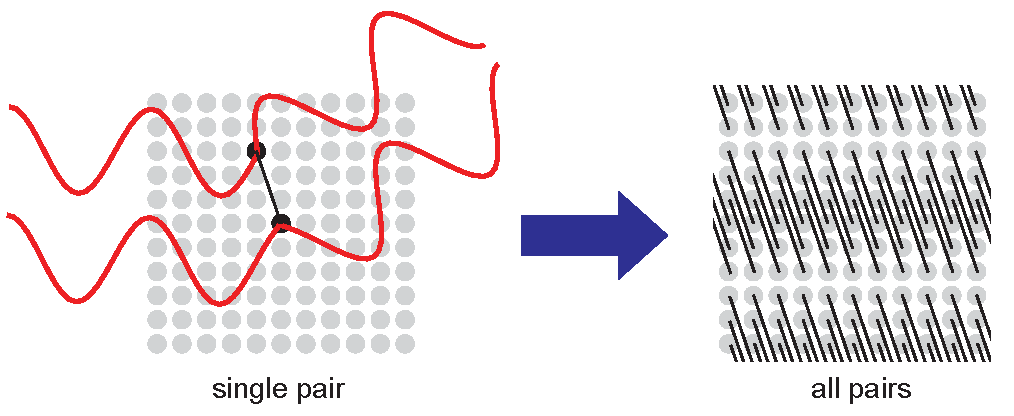
\includegraphics[width=0.75\textwidth]{\figpath/Model1_pairing}}
	
\end{model}


\begin{ctqs}
	
	\question Will any scattered intensity be observed in a light scattering measurement on a perfectly homogeneous sample?  Why or why not?  Explain your group's reasoning in 1-2 complete sentences.
	
		\begin{solution}[1.5in]{}
		
			No.  When the medium is homogeneous, all molecules have a partner that is exactly the right distance away to lead to destructive interference in the scattered light.  As a result, all of the scattered light will destructively interfere and no intensity will be measured on the detector.
			
			\emph{Note: in discussion, it is worth noting that this argument holds primarily when the distance between scattering centers is much smaller than the wavelength of light being used in the experiment.  In this case, the scattering process is a so-called ``incoherent'' scattering process.}
			
		\end{solution}

	\question Suppose one of the molecules is moved, as shown below.
	
	\vspace{6pt}
	\centerline{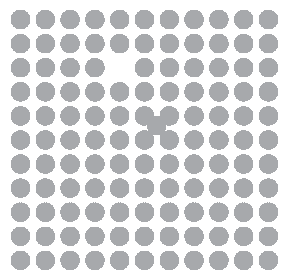
\includegraphics[width=0.2\textwidth]{\figpath/Model1_displacement}}

		\begin{enumerate}
			\item Do the molecules all still have ``partners'' that are the right distance away to scatter light with perfect destructive interference? 
	
		\begin{solution}[0.5in]{}
			no
		\end{solution}
			
			\item Will any scattered intensity be observed in a light scattering measurement on this sample?  Why or why not?  Explain your group's reasoning in 1-2 complete sentences.
	
		\begin{solution}[1in]{}
			Yes, now scattered intensity might be observed. The molecule that was ``partnered'' with the molecule that moved no longer has a partner that is in the right position to scatter destructively with it, and the molecule that moved also does not have a partner (because all of the other molecules are already paired up).  As such, some of the scattered light will not be canceled out by destructive interference with light scattered by other molecules, and some intensity might be observed at the detector.
		\end{solution}
			
		\end{enumerate}
		
	\question Several possible distributions of molecules in a sample are shown below: \label{\labelbase:ctq:fluctuations}
	
	\centerline{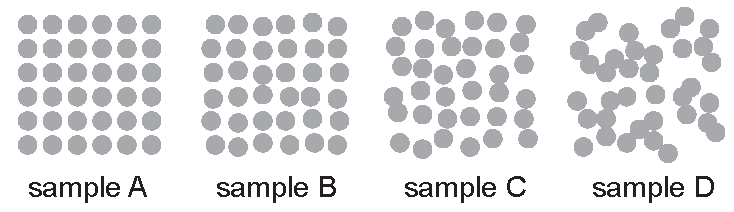
\includegraphics[width=0.5\textwidth]{\figpath/Model1_fluctuation}}
	
		Which of these samples would you expect to give the \emph{highest} intensity of scattered light?  Explain your group's reasoning in 1-2 complete sentences.
	
		\begin{solution}[1in]{}
			Sample D should give the highest intensity of scattered light, because it has the least homogeneous distribution of molecules/scattering centers, so will have the least ``pairing up'' of molecules to give scattering signals that interfere destructively.
		\end{solution}

\end{ctqs}

\begin{infobox}
	It is possible to show that the excess scattering from a polymer sample ($\frac{I_{ex}}{I_0}$) is related to the size of the concentration fluctuations in cells of volume $\Psi$ by
	\begin{equation*}
		\frac{I_{ex}}{I_0} = \frac{4 \pi^2 n^2 \Psi}{r^2 \lambda^4}\left(\frac{\partial n}{\partial c}\right)^2_{T,p} \langle ( \delta c )^2 \rangle
	\end{equation*}
	Here, $\delta c$ is the size of the concentration fluctuations,  $\frac{d n}{dc}$ is the change in the refractive index,  $n$, of the mixture with changes in the solute concentration, $c$ (where $c$ is measured in units of mass of solute per unit volume), and $r$ is the distance from the sample to the detector.
\end{infobox}

\begin{ctqs}

	\question Is this expression consistent with your answer to CTQ \ref{\labelbase:ctq:fluctuations}?  Briefly explain how you know.
	
		\begin{solution}[1in]{}
		
			Yes, this equation is qualitatively consistent with the answer to CTQ \ref{\labelbase:ctq:fluctuations}, because it predicts that the sample with the largest average concentration fluctuations ($\langle \delta c\rangle$) should give the highest scattering intensity.
			
		\end{solution}
	
\end{ctqs}

\begin{model}[Equilibrium Fluctuations \& Static Light Scattering]
	\label{\labelbase:mdl:SLS}

Changes in polymer concentration typically change the free energy of the mixture, as shown below.
	
	\centerline{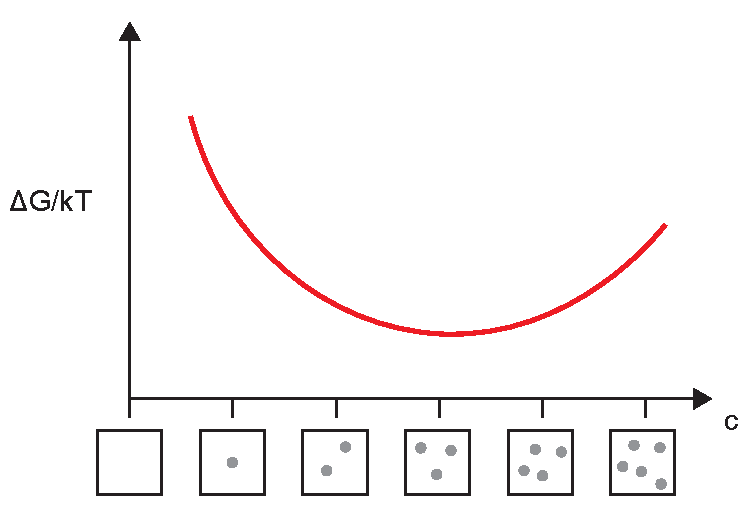
\includegraphics[width=0.4\textwidth]{\figpath/Model1_deltaG}}
	
\end{model}

\begin{ctqs}
	
		\question Which of the following two states has the higher free energy?
	
	\vspace{6pt}
	\centerline{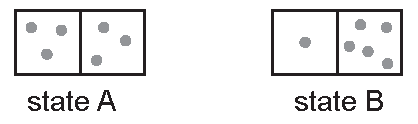
\includegraphics[width=0.25\textwidth]{\figpath/Model1_twostates}}
	
			\begin{solution}[0.25in]{}
				State B
			\end{solution}
			
		\question For which of the following free energy curves will it be ``easiest'' to go from state A to state B?  Briefly explain your reasoning.  \label{\labelbase:ctq:delGcurvature}
	
	\centerline{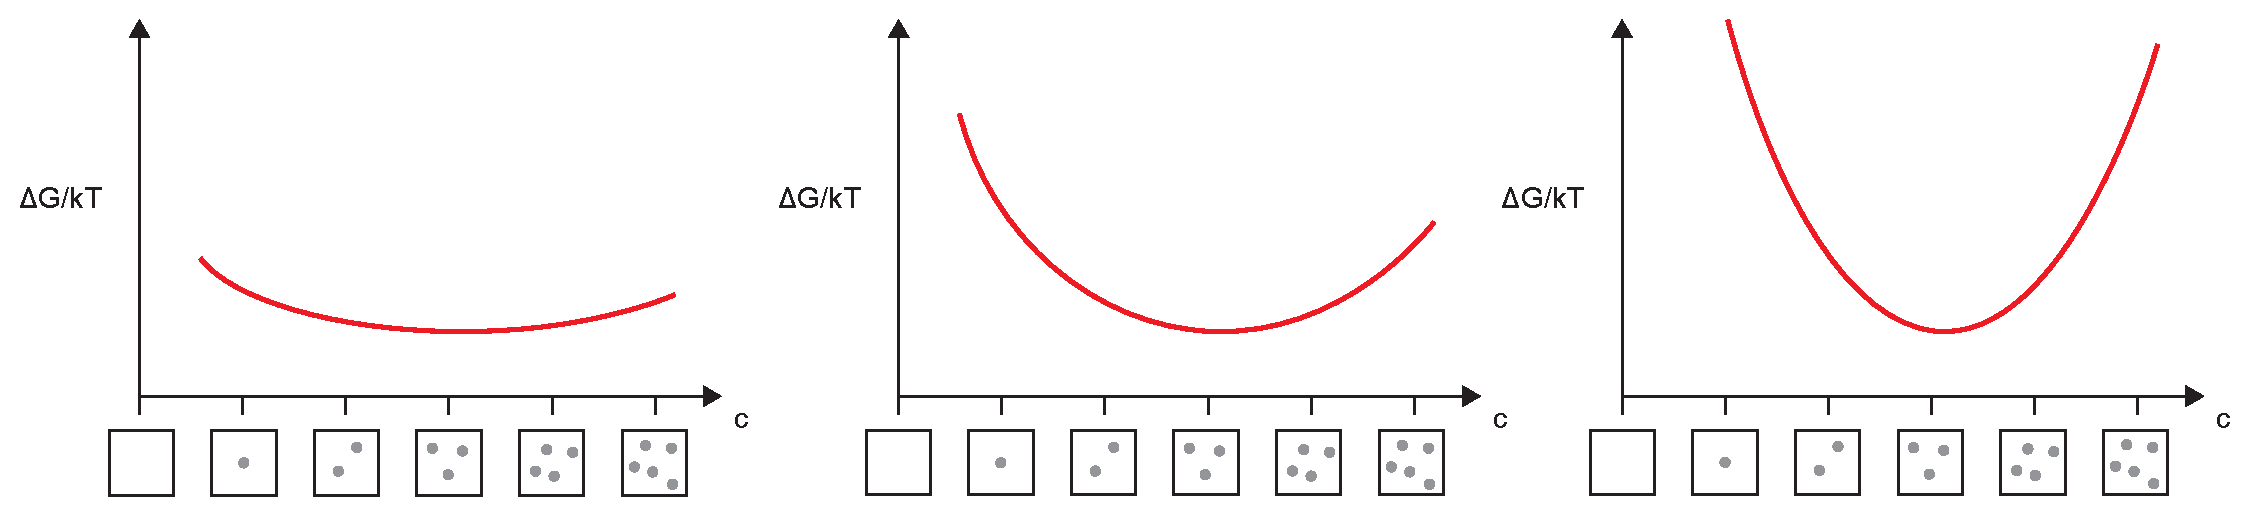
\includegraphics[width=0.75\textwidth]{\figpath/Model1_curvature}}
	
			\begin{solution}[1in]{}
				It should be easiest to go from state A to state B for the curve on the left.  This curve has the lowest curvature and the smallest free energy penalty for going from state A to state B.
			\end{solution}
			
	\question If the temperature of the system is increased, will it be easier or harder to go from state A to state B?  Briefly explain your reasoning. \label{\labelbase:ctq:temperature}
	
			\begin{solution}[1in]{}
				Increasing the temperature will make it easier to go from state A to state B, because it increases the energy available to move ``up'' the curve.
			\end{solution}
	
\end{ctqs}

\begin{infobox}
	It is possible to show that the average size of the concentration fluctuations across cells of volume $\Psi$ is
	\begin{equation*}
		\langle (\delta c)^2\rangle = \frac{k_BT}{\left( \frac{\partial^2 G}{\partial c^2}\right)_{T,p}} \approx \left(\frac{c}{\Psi N_{av}}\right) \left(\frac{1}{1/M_w + 2Bc}\right)
	\end{equation*}
	where $M_w$ is the weight-average molecular weight of the polymer and $B$ is the so-called ``second virial coefficient'' which reflects how much the polymer chains do or do not prefer to be near other polymers in solution.
\end{infobox}

\begin{ctqs}
	\question Is this expression consistent with the behavior you predicted in CTQs \ref{\labelbase:ctq:delGcurvature} and \ref{\labelbase:ctq:temperature}?  Briefly explain how you know.
	
		\begin{solution}[1.5in]{}
		
			Yes, this equation is consistent with the answers to CTQs \ref{\labelbase:ctq:delGcurvature} and \ref{\labelbase:ctq:temperature}.  In the middle expression, the temperature is in the numerator, so increasing the temperature increases the average size of the concentration fluctuations, $\langle (\delta c)^2\rangle$.  The second derivative of the free energy is in the denominator, so lowering the curvature of the free energy curve makes the denominator smaller and also increases the value of $\langle (\delta c)^2\rangle$.
			
			\emph{Note: if you did the activities on Flory-Huggins theory and phase behavior of polymer solutions, you may mention in discussion that $B$ is related to the interaction parameter, $\chi$ - see e.g. Hiemenz \& Lodge section 7.4.2 for details.}
		\end{solution}

	\question Combine the equations from the two preceding Information boxes to obtain one (messy!) equation for $I_{ex}/I_0$.   Don't worry about simplifying it, but do verify that the $\Psi$ terms cancel out.
	
		\begin{solution}[1.5in]{}
			\begin{align*}
				\frac{I_{ex}}{I_0} &= \frac{4 \pi^2 n^2 \Psi}{r^2 \lambda^4}\left(\frac{\partial n}{\partial c}\right)^2_{T,p} \frac{c}{\Psi N_{av}} \frac{1}{1/M_w + 2Bc} \\
				&= \frac{4 \pi^2 n^2}{r^2 \lambda^4}\left(\frac{\partial n}{\partial c}\right)^2_{T,p} \frac{c}{ N_{av}} \frac{1}{1/M_w + 2Bc}
			\end{align*}
		\end{solution}
		
	\question It is usually convenient to group all of the constants into a single optical constant, $K$, where
		\begin{equation*}
			K = \frac{4\pi^2 n^2 (\partial n / \partial c)^2}{\lambda^4 N_{av}}
		\end{equation*}
		Rewrite your expression for $\frac{I_{ex}}{I_0}$ in terms of the optical constant $K$, the concentration of the polymers $c$, their molecular weight $M_w$, and the second virial coefficient, $B$.
		
		\begin{solution}[1in]{}
			\begin{equation*}
				\frac{I_{ex}}{I_0} = \frac{Kc}{r^2} \frac{1}{1/M_w + 2Bc}
			\end{equation*}
		\end{solution}
	
	\question It is also often most convenient to work in terms of the \emph{Rayleigh ratio}, $R_\theta = \frac{r^2 I_{ex}}{I_0}$.  Rearrange your answer from the previous question to obtain an expression for $R_\theta$.
		
		\begin{solution}[0.75in]{}
			\begin{equation*}
				R_\theta = r^2 \frac{I_{ex}}{I_0} = \frac{Kc}{1/M_w + 2Bc }
			\end{equation*}
		\end{solution}
	
	
\end{ctqs}

\begin{infobox}

	Polymers are not quite point particles, so the light scattered from each polymer chain in the sample has a small dependence on $q$.  If $qR_g < 1$, then the $q$-dependence is given by the form factor,
	\begin{equation*}
		P(q) = 1 - \frac{q^2}{3}R_g^2 + \dots
	\end{equation*}
	where the $\dots$ indicate higher-order terms in $q$ (e.g. terms that go as $q^4$, $q^6$, etc.).	
	Combining this equation with the expression you obtained in the previous question, we find that
	\begin{equation*}
		\frac{Kc}{R_\theta} = \frac{1}{M_w}\left( 1 + \frac{q^2}{3} R_g^2 + \dots \right) + 2Bc + \dots
	\end{equation*}
	This is the \emph{Zimm equation}.
\end{infobox}

\begin{ctqs}
	
	\question When $c$ is very small,
		\begin{equation*}
			\frac{Kc}{R_\theta} \approx \frac{1}{M_w}\left(1 + \frac{q^2}{3}R_g^2 + \dots\right)
		\end{equation*}
		In this equation...
		\begin{enumerate}
				
			\item Which variable contains information about the scattering angle?
			
				\begin{solution}[0.25in]{}
					$q$
				\end{solution}
				
			\item Which variable contains information about the intensity of the scattered light?
			
				\begin{solution}[0.25in]{}
					$R_\theta$
				\end{solution}
				
		\end{enumerate}
		
	\question Propose a method that you could use to determine \emph{both} the weight-average molecular weight \emph{and} the radius of gyration of a polymer from data about how the intensity of light scattered from a dilute polymer solution changes with scattering angle.
		
		\begin{solution}[1.5in]{}
			You could measure the scattered intensity as a function of scattering angle.  Then, you could calculate $R_\theta$ and $q$ for each angle, plot $\frac{Kc}{R_\theta}$ vs $q^2$ and perform a linear fit.  The intercept of this fit would be $\frac{1}{M_w}$ and the slope would be $\frac{R_g^2}{3M_w}$, so once you know both the slope and the intercept, you can solve for $R_g$ and $M_w$.
		\end{solution}
		
	\question If you wanted to additionally obtain information about the second virial coefficient, $B$, how could you modify your proposed experiment?  Explain your reasoning in 1-2 complete sentences.
		
		\begin{solution}[1.5in]{}
			To obtain information about $B$, you would need to measure multiple samples with different polymer concentrations, $c$.  At $q=0$, the Zimm equation becomes
			\begin{equation*}
				\frac{Kc}{R_\theta} = \frac{1}{M_w} + 2Bc + ...
			\end{equation*}
			so a plot of $\frac{Kc}{R_\theta}$ vs $c$ would have a slope equal to $2B$.
			
			Note: In practice, we cannot measure right at $q=0$, so we usually measure multiple samples with different concentrations at multiple scattering angles. We then extrapolate the angle-dependent data to $q=0$ and fit the extrapolated $q=0$ data to obtain $B$.  This is typically shown on a \textit{Zimm plot}.
		\end{solution}
		
\end{ctqs}


\begin{model}[Time-Dependent Fluctuations and Dynamic Light Scattering]
	\label{\labelbase:mdl:DLS}
	
	In Model \ref{\labelbase:mdl:SLS}, above, we considered only the \emph{average} intensity of the light scattered from a polymer solution.   However, the distribution of molecules (and the scattered intensity) can also change with time.
	
	Shown below are the distributions of molecules that might be present in a polymer solution at a series of different times, $t$:
	
	\vspace{6pt}
	\centerline{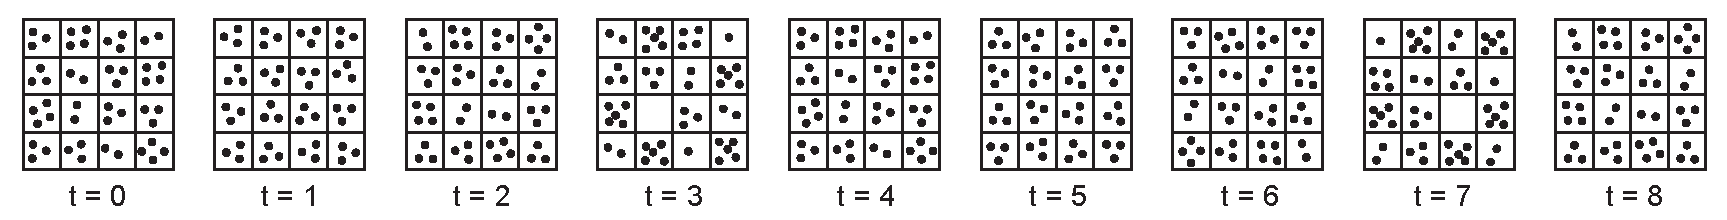
\includegraphics[width=\textwidth]{\figpath/Model2_fluctuations_medium}}
	
\end{model}

\begin{ctqs}

	\question At which times are the concentrations of molecules at different positions in the solution...
	
		\begin{enumerate}
			\item ... very similar?
			
				\begin{solution}[0.25in]{}
					$t=1$ and $t=5$
				\end{solution}
			
			\item ... very different?
			
				\begin{solution}[0.25in]{}
					$t=3$ and $t=7$
				\end{solution}
		\end{enumerate}
		
	\question At which times will the solution...
	
		\begin{enumerate}
			\item ... scatter a lot of light?
			
				\begin{solution}[0.25in]{}
					$t=3$ and $t=7$ (i.e. when the concentration fluctuations are large)
				\end{solution}
			
			\item ... scatter little light?
			
				\begin{solution}[0.25in]{}
					$t=1$ and $t=5$ (i.e. when the concentration fluctuations are small)
				\end{solution}
				
		\end{enumerate}
		
		\clearpage
	\question On the following axes, sketch the intensity of the scattered light that you would expect to measure from this solution as a function of time:
	
		\vspace{6pt}
		\begin{solution}[0.75in]{\centerline{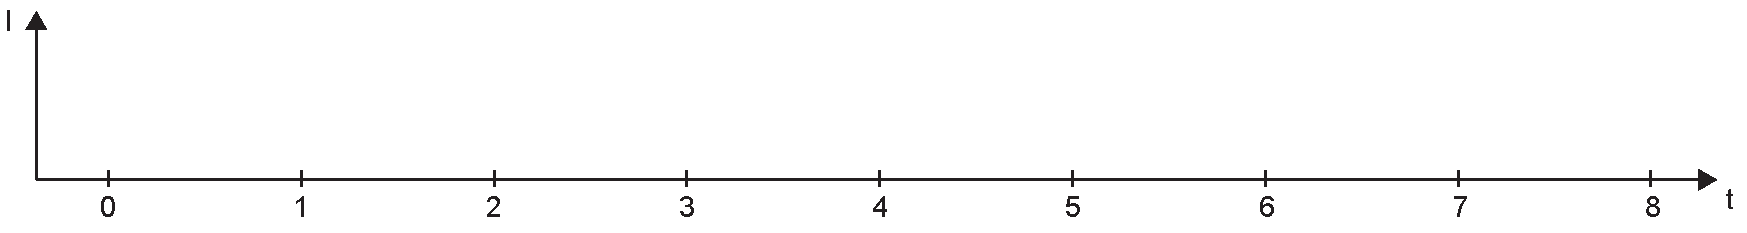
\includegraphics[width=0.9\textwidth]{\figpath/Model2_Is_blank}}}
		\centerline{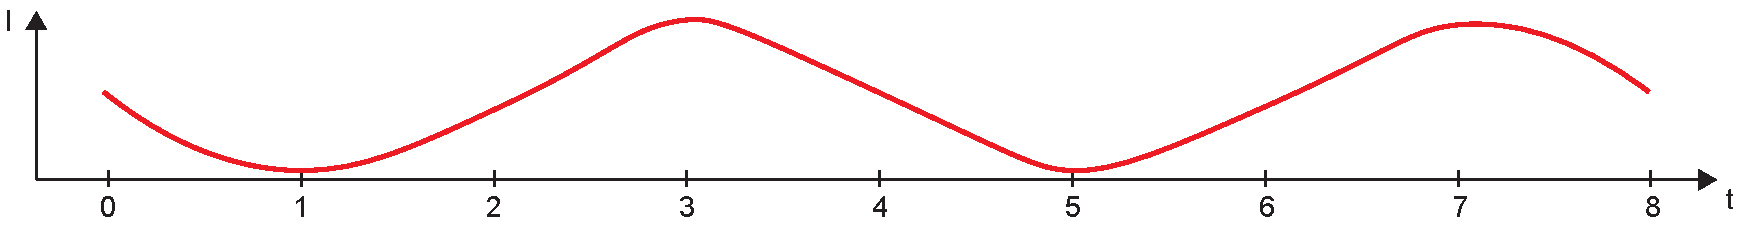
\includegraphics[width=0.9\textwidth]{\figpath/Model2_fluctuations_medium_solution}}
		\end{solution}
		\vspace{6pt}
		
	\question The time-dependent distributions of molecules in two different solutions are shown below.  For each solution, sketch the intensity of the scattered light that you would expect to measure from the solution as a function of time.
	
		\begin{enumerate}
			\item Solution A:
			
			\vspace{6pt}
			\begin{solution}[1.5in]{
			\centerline{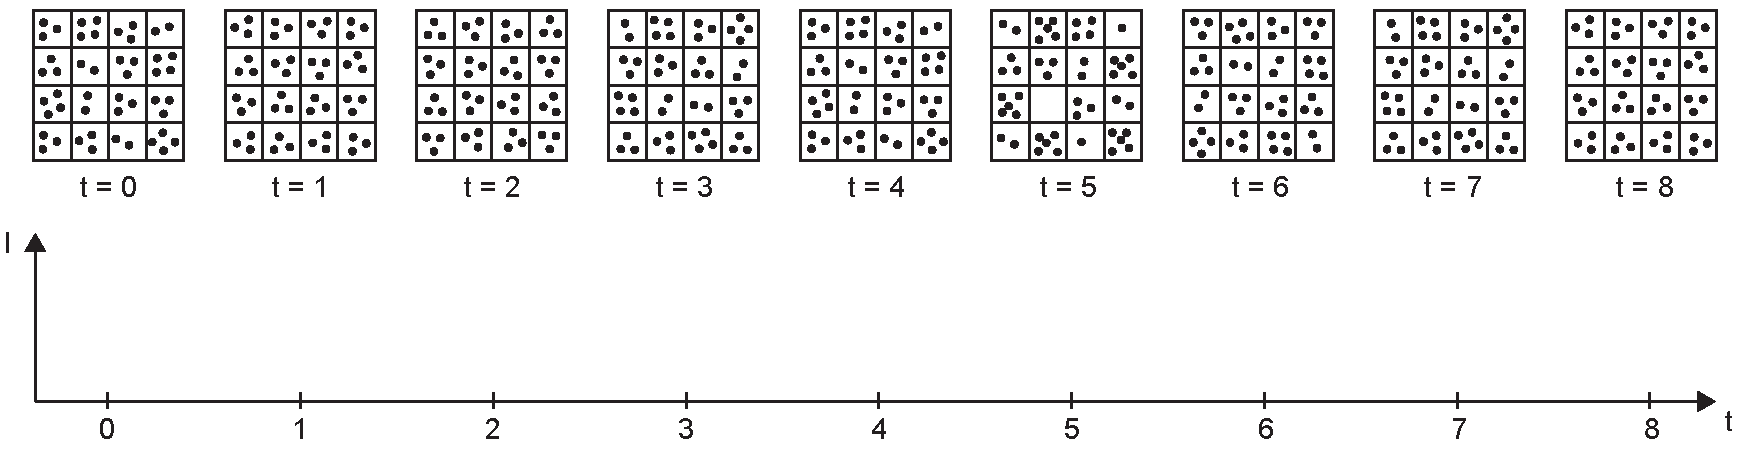
\includegraphics[width=\textwidth]{\figpath/Model2_fluctuations_slow}}}
			\centerline{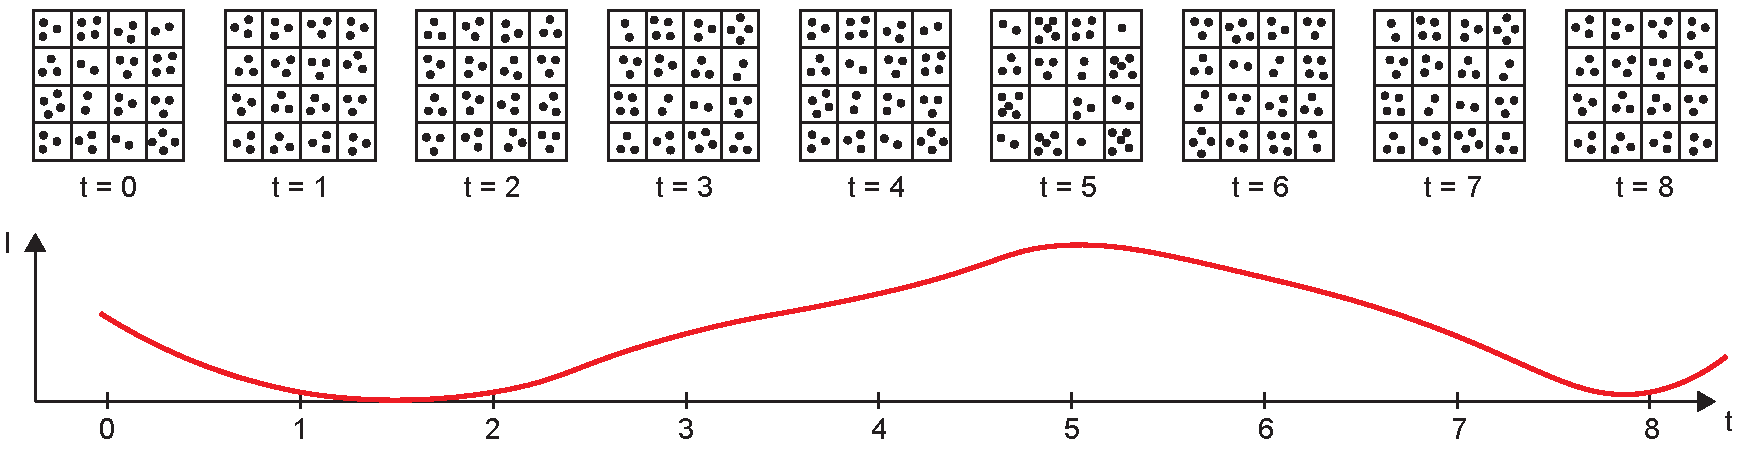
\includegraphics[width=\textwidth]{\figpath/Model2_fluctuations_slow_solution}}
			\end{solution}
			\vspace{6pt}
			
			\item Solution B:
			
			\vspace{6pt}
			\begin{solution}[1.5in]{
			\centerline{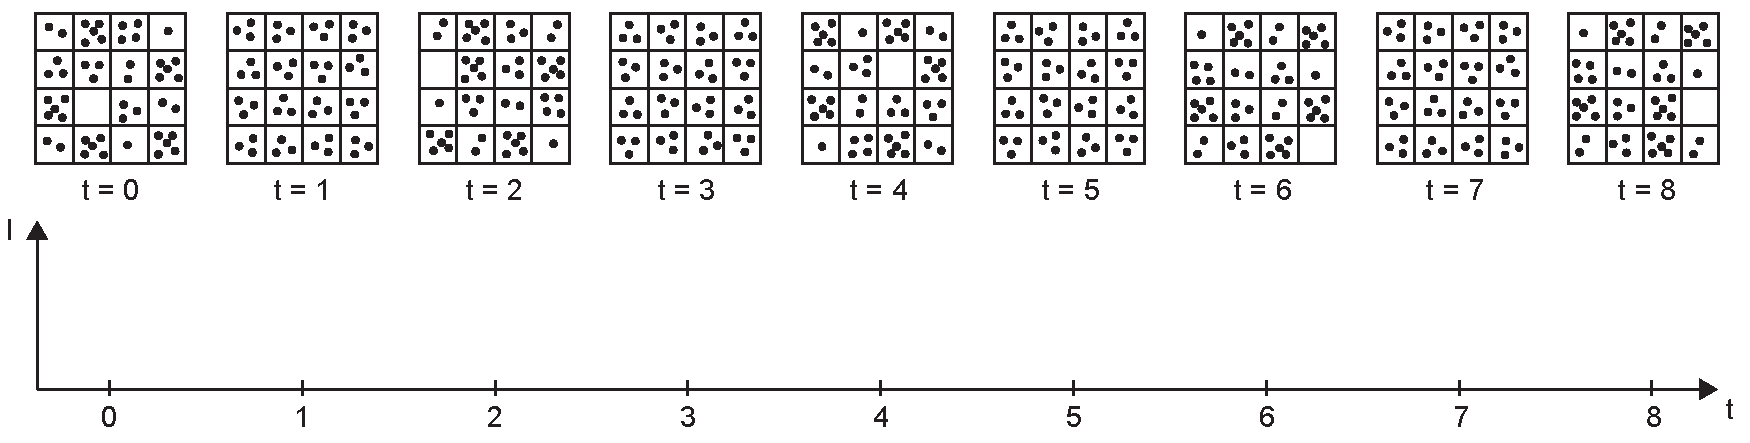
\includegraphics[width=\textwidth]{\figpath/Model2_fluctuations_fast}}}
			\centerline{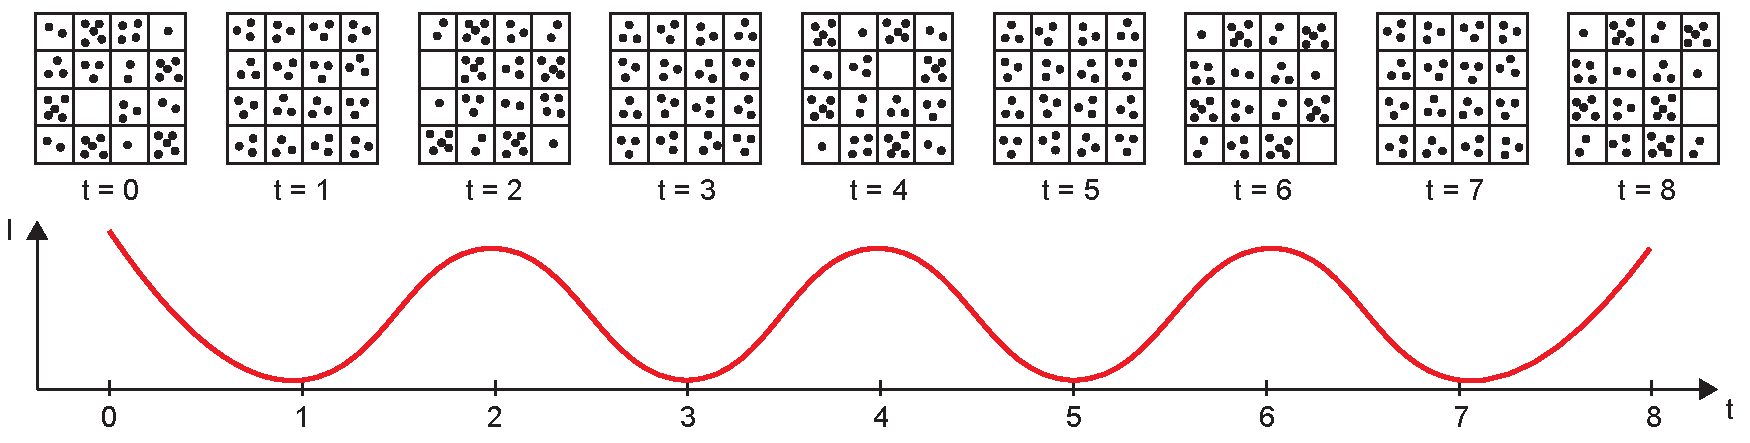
\includegraphics[width=\textwidth]{\figpath/Model2_fluctuations_fast_solution}}
			\end{solution}
		\end{enumerate}
		
	\question In which of the solutions shown above do you think the molecules were probably diffusing \emph{fastest}?  Explain your group's reasoning in 1-2 complete sentences.
	
		\begin{solution}[1.5in]{}
			The molecules were probably diffusing fastest in solution B.  If the molecules move faster, concentration fluctuations can happen more quickly.
			
			\emph{Note: as drawn, the intensity fluctuations are all roughly periodic.  In discussion, it may be worth noting that the intensity fluctuations are in actuality much more random, and briefly explain what an autocorrelation function is and why it gives information about how long the sample ``remembers'' its previous configuration.}
			
			\emph{To motivate the $q$ dependence of $C(t)$ on the next page, you may also mention that the $q$ dependence comes from the timescale required for concentration fluctuations to occur on length scales comparable to $1/q$.}
		\end{solution}
	
\end{ctqs}

\clearpage
\begin{infobox}
	The timescales over which the scattered intensities change can be characterized using the \textit{intensity autocorrelation function},
	\begin{equation*}
		C(t) = \int I_s(t') I_s(t'+t)dt'
	\end{equation*}
	For molecules diffusing with diffusion coefficient $D$, the intensity autocorrelation function measured at scattering vector $q$ has the form
	\begin{equation*}
		C(t) = A e^{-2 q^2 D t} + B
	\end{equation*}
\end{infobox}

\begin{ctqs}
	\question The intensity autocorrelation functions obtained from three different samples are shown below.
	
			\vspace{6pt}
			\centerline{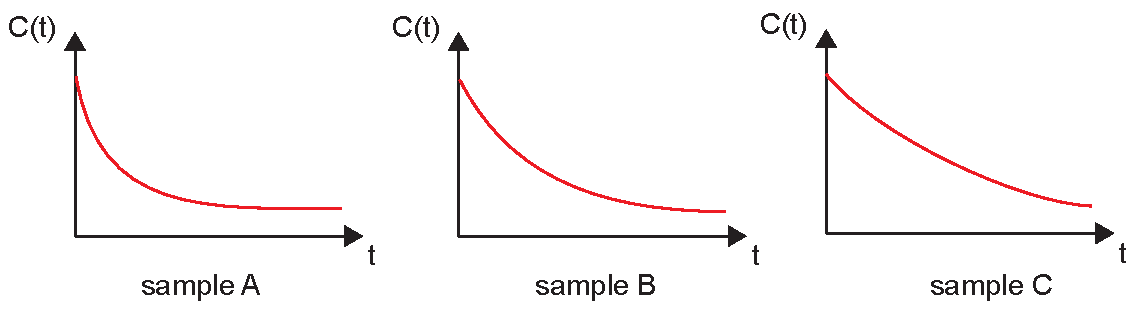
\includegraphics[width=0.7\textwidth]{\figpath/Model2_correlationfunctions}}	
	
		If all three samples were measured at the same scattering angle, in which sample were the particles diffusing the fastest?  Explain your reasoning in 1-2 complete sentences.
	
		\begin{solution}[1.25in]{}
			The decay is fastest in sample A.  A faster decay occurs when the magnitude of $2q^2 D$ in the exponent of $C(t)$ is larger, so a faster decay corresponds to a larger diffusion constant (faster diffusion of the particles).
		\end{solution}
	
	\question The diffusion coefficient of spherical particles with radius $R$ in a solvent with viscosity $\eta_s$ is given by the Stokes-Einstein relation,
	\begin{equation*}
		D = \frac{ k_B T}{6\pi \eta_s R}
	\end{equation*}
	Based on this relationship, in which of the samples in the preceding question must the particles have been the \emph{largest}?  Explain your reasoning in 1-2 complete sentences. \label{\labelbase:ctq:stokeseinstein}
	
		\begin{solution}[1.25in]{}
			The particles must have been the largest in sample C.  A larger value of $R$ \textit{decreases} the value of D, which in turn makes the exponential decay in $C(t)$ occur more slowly.  $C(t)$ has the slowest decay for sample C, so sample C must have contained the largest particles.
		\end{solution}
	
	\question Summarize, in your own words, how you could determine the effective radius of a polymer in solution from data about how the scattering intensity varies with time.
	
		\begin{solution}[1.5in]{}
			To determine the effective radius of a particle in solution, you would need to measure the scattering intensity as a function of time at a known angle or scattering vector $q$, compute the autocorrelation function, and fit it to an exponential decay.  The decay constant could then be used to calculate the diffusion coefficient, and the diffusion coefficient could be used to calculate the effective radius of the polymer.
			
			%\emph{Note: most benchtop DLS measurements measure only at a single angle, i.e. a single $q$ value.  Research instruments using goniometer systems, however, can measure at multiple angles; the decay constants at each angle can then be plotted against $q^2$ and fit to obtain a more accurate value of $D$.}
		\end{solution}

\end{ctqs}



\begin{exercises}

	\exercise The Stokes-Einstein relation, as given in CTQ \ref{\labelbase:ctq:stokeseinstein}, assumes that the particle is a perfect sphere.
	
		\begin{enumerate}
		
			\item Are polymer chains perfectly spherical particles?  If not, how would you interpret the value of $R$ obtained in a dynamic light scattering experiment?  Explain why we typically refer to radii measured in this way as ``hydrodynamic'' radii.
			
				\begin{solution}{}
					No, polymer chains are not perfectly spherical.  The value of $R$ obtained in a dynamic light scattering experiment should be interpreted as the radius of a sphere that has the same diffusion constant as the polymer chain of interest.
					
					We call it the ``hydrodynamic'' radius because it is the essentially reflecting the average ``drag'' experienced by the polymer as it moves through the fluid.  Movement through a fluid is a dynamic process, and ``hydro'' is a prefix meaning water (or more generally, fluid); hence the hydrodynamic radius is the radius that reflects the dynamics of a particle's movement through a fluid.

				\end{solution}
			
			\item Is the hydrodynamic radius ($R_h$) of a polymer chain obtained in a dynamic light scattering experiment likely to be bigger or smaller than its radius of gyration ($R_g$)?  Explain your reasoning in 1-2 complete sentences.
			
				\begin{solution}{}
				
				To a first approximation, for a polymer that is well-described as a Gaussian coil in solution, $R_h$ should usually be smaller than $R_g$.  This is because most of the polymer coil is actually empty space, and solvent can ``drain'' through the coil as the chain moves.  As such, the chain does not have to displace as much solvent as a solid sphere of the same size would, so it indeed diffuses faster than a solid sphere with the same nominal radius.

There are two caveats to this statement, however:

First, the polymer coil does extend further into the solution than its radius of gyration – remember that $R_g$ is a measure of average distance of monomers from the center of mass, so some will be much closer in and some will be much further out.  On average, a loose coil will still diffuse faster than a solid sphere with a radius equal to the polymer's $R_g$, but this should in no way be interpreted as saying that the polymer is ``smaller'' than $R_g$.

Second, even for a solid sphere, $R_h$ is not equal to $R_g$!  This is because, again, $R_g$ is a measure of the average distance of the pieces of the particle from its center of mass, and $R_g$ is actually smaller than $R$ for solid spheres.  This means that for a solid sphere, $R_h > R_g$, or exactly the opposite of what we stated above for the loose Gaussian coil.  So, the conformation of the polymer chains plays an important role in determining the relationship between $R_g$ and $R_h$.


				\end{solution}
			
		\end{enumerate}
	
\end{exercises}


%\begin{problems}
%
%	\problem First exercise
%	\problem Second exercise
%	
%\end{problems}


	
\end{activity}